% Options for packages loaded elsewhere
\PassOptionsToPackage{unicode}{hyperref}
\PassOptionsToPackage{hyphens}{url}
%
\documentclass[
]{article}
\title{Project Regression Methods - 2022}
\author{Céline Guex - sciper n°310673, Candice Baud - sciper n°359523}
\date{20 décembre 2022}

\usepackage{amsmath,amssymb}
\usepackage{lmodern}
\usepackage{iftex}
\ifPDFTeX
  \usepackage[T1]{fontenc}
  \usepackage[utf8]{inputenc}
  \usepackage{textcomp} % provide euro and other symbols
\else % if luatex or xetex
  \usepackage{unicode-math}
  \defaultfontfeatures{Scale=MatchLowercase}
  \defaultfontfeatures[\rmfamily]{Ligatures=TeX,Scale=1}
\fi
% Use upquote if available, for straight quotes in verbatim environments
\IfFileExists{upquote.sty}{\usepackage{upquote}}{}
\IfFileExists{microtype.sty}{% use microtype if available
  \usepackage[]{microtype}
  \UseMicrotypeSet[protrusion]{basicmath} % disable protrusion for tt fonts
}{}
\makeatletter
\@ifundefined{KOMAClassName}{% if non-KOMA class
  \IfFileExists{parskip.sty}{%
    \usepackage{parskip}
  }{% else
    \setlength{\parindent}{0pt}
    \setlength{\parskip}{6pt plus 2pt minus 1pt}}
}{% if KOMA class
  \KOMAoptions{parskip=half}}
\makeatother
\usepackage{xcolor}
\IfFileExists{xurl.sty}{\usepackage{xurl}}{} % add URL line breaks if available
\IfFileExists{bookmark.sty}{\usepackage{bookmark}}{\usepackage{hyperref}}
\hypersetup{
  pdftitle={Project Regression Methods - 2022},
  pdfauthor={Céline Guex - sciper n°310673, Candice Baud - sciper n°359523},
  hidelinks,
  pdfcreator={LaTeX via pandoc}}
\urlstyle{same} % disable monospaced font for URLs
\usepackage[margin=1in]{geometry}
\usepackage{graphicx}
\makeatletter
\def\maxwidth{\ifdim\Gin@nat@width>\linewidth\linewidth\else\Gin@nat@width\fi}
\def\maxheight{\ifdim\Gin@nat@height>\textheight\textheight\else\Gin@nat@height\fi}
\makeatother
% Scale images if necessary, so that they will not overflow the page
% margins by default, and it is still possible to overwrite the defaults
% using explicit options in \includegraphics[width, height, ...]{}
\setkeys{Gin}{width=\maxwidth,height=\maxheight,keepaspectratio}
% Set default figure placement to htbp
\makeatletter
\def\fps@figure{htbp}
\makeatother
\setlength{\emergencystretch}{3em} % prevent overfull lines
\providecommand{\tightlist}{%
  \setlength{\itemsep}{0pt}\setlength{\parskip}{0pt}}
\setcounter{secnumdepth}{5}
\usepackage{booktabs}
\usepackage{longtable}
\usepackage{array}
\usepackage{multirow}
\usepackage{wrapfig}
\usepackage{float}
\usepackage{colortbl}
\usepackage{pdflscape}
\usepackage{tabu}
\usepackage{threeparttable}
\usepackage{threeparttablex}
\usepackage[normalem]{ulem}
\usepackage{makecell}
\usepackage{xcolor}
\ifLuaTeX
  \usepackage{selnolig}  % disable illegal ligatures
\fi

\begin{document}
\maketitle

\hypertarget{introduction---summary}{%
\section{Introduction - Summary}\label{introduction---summary}}

This report describes the analysis of three databases on events in
French motorway tunnels.\\
The data shows \ldots{} to do after our analysis.

\hypertarget{initial-data-analysis}{%
\section{Initial data analysis}\label{initial-data-analysis}}

\hypertarget{description-of-fires-dataset}{%
\subsection{Description of Fires
dataset}\label{description-of-fires-dataset}}

This data set lists fires that occurred in French tunnels. The data set
gathers 92 tunnels ran by 25 companies. Many parameters are also
registered, like traffic, proportion of trucks among tunnel's users (in
\%), length of the tunnel, maximum speed allowed,slope inclination in
the tunnel (in \%), shape of the tunnel (slope type in the tunnel) and
situation of the tunnel (if it lies in urban area or not). Some tunnels
are unidirectional and some are bidirectional. We will use this data set
to determine the factors that are the most likely to yields to fires in
tunnel. We will also look for factors that might reduce the risk of
fires.\\

Figure 1 shows the distribution of the fires with a fitted poisson
distribution, and the correlations between the different variables.\\

REMARK : I wanted to put them side by side with par but it doesn't seem
to work.\\

\begin{verbatim}
## `stat_bin()` using `bins = 30`. Pick better value with `binwidth`.
\end{verbatim}

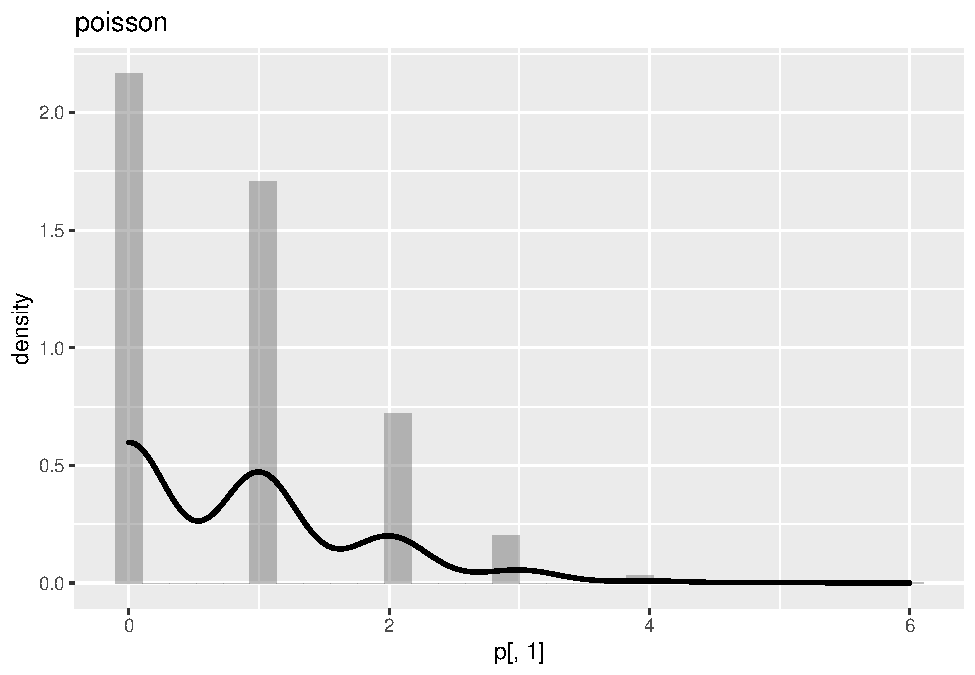
\includegraphics{Report_files/figure-latex/exploratory-1.pdf}
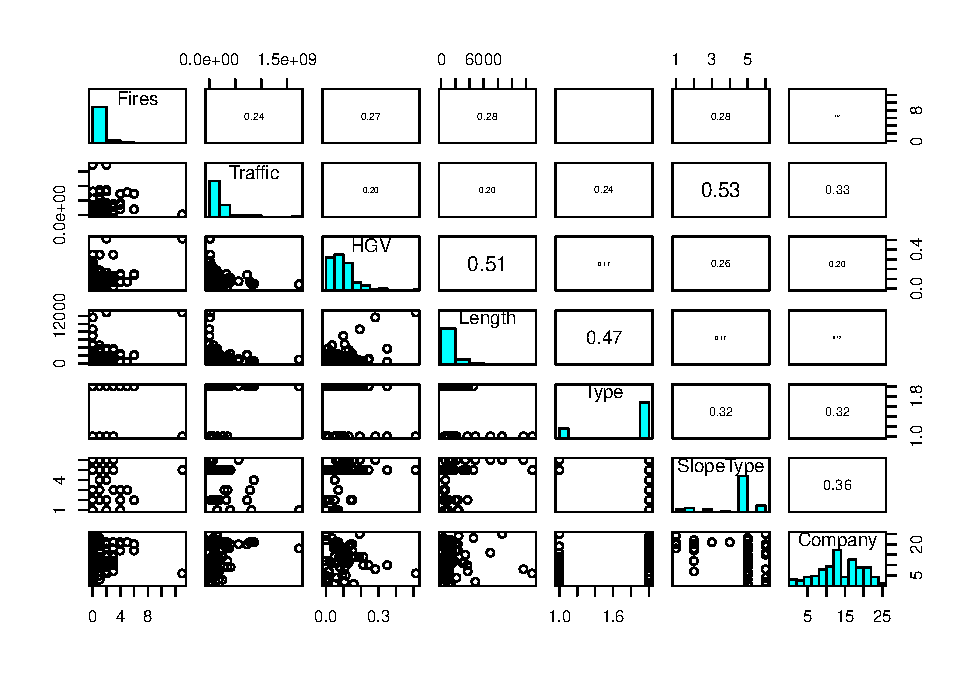
\includegraphics{Report_files/figure-latex/exploratory-2.pdf} From the
correlation plot, it is clear that the variables that seem to be the
most explanatory are Length, HGV and Traffic. Moreover, Length is also
strongly correlated with HGV. Finally, Limit is also significatively
correlated with HGV.\\

BROUILLON en français : traffic length hgv et slopetype sont les plus
corrélées avec fires. Company je l'ai laissé parce que c'est corrélé
avec traffic et slopetype donc c'est intéressant. length et HGV
corrélées intéressant. Slopetype et traffic corrélées intéressant.

REMARK : I was thinking of then plot length with HGV, and LImit with HGV
and fit a regression to see a bit how the variables are linked.\\

From this exploratory analysis, we will try to fit a Poisson model.\\
REMARK : put some equations as in his report ? or we put them after ?\\

\hypertarget{description-of-accidents-dataset}{%
\subsection{Description of Accidents
dataset}\label{description-of-accidents-dataset}}

The accidents dataset gathers contains 92 tunnels ran by 25 companies.
The variables from the dataset Fires are also present in the Accidents
one. But the latter also includes the Year in which the accidents
occurred, the width of lanes in the tunnel in metres (variable Width)
and the number of lanes in the tunnel (variable Lanes).\\

Figure 2 shows the distribution of the fires with a fitted exponential
distribution, and the most relevant correlations between the different
variables. We chose to represent only the variables that had a
correlation greater than 0.25.\\

\begin{verbatim}
## `stat_bin()` using `bins = 30`. Pick better value with `binwidth`.
\end{verbatim}

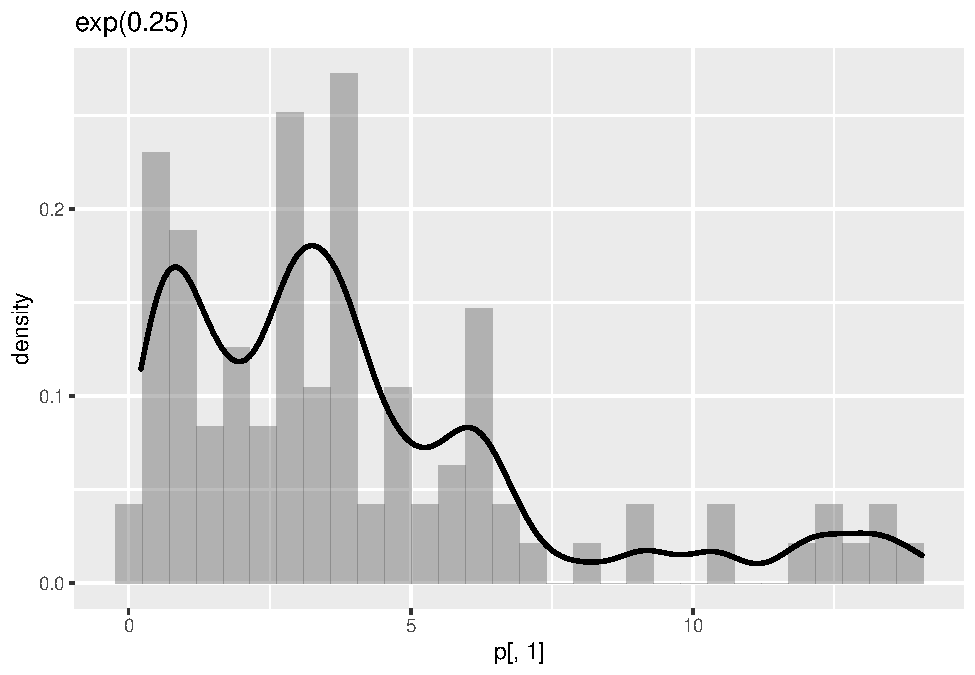
\includegraphics{Report_files/figure-latex/Accidents corr and fit-1.pdf}
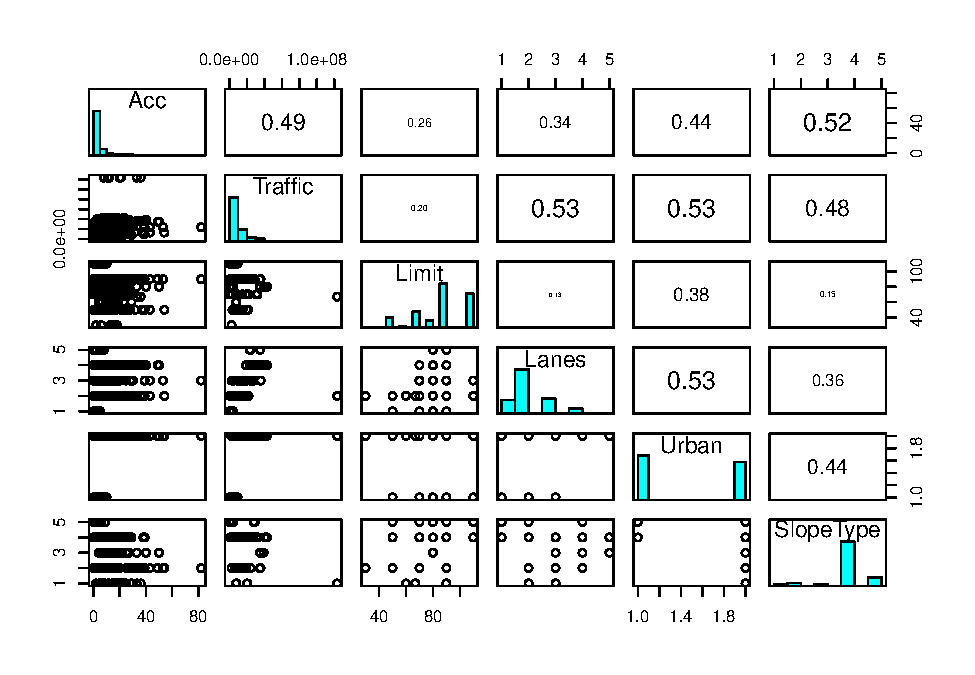
\includegraphics{Report_files/figure-latex/Accidents corr and fit-2.pdf}
What one clearly sees from the correlation plot is that Accidents are
mostly correlated with Traffic, which seems intuitive since the more
people on the road, the most accidents can occur. The second most
correlated variable is SlopeType which can take values : Continuous
slope, Basin, Other, Roof, Unknown. Intuitively, we conclude that
according to the SlopeType, the dangerousness of the tunnel won't be the
same. One thing to notice however is that SlopeType and Traffic are also
quite strongly correlated (0.48), which means that depending on the
slope type, the affluence might differ which can in the end impact the
number of accidents. The same thing occurs for the Urban variable.
Indeed, Urban is quite strongly correlated with the number of accidents
but also with the traffic and the slope type.\\

Comment : Include Limit?? Maybe we can just show the 5 more relevant ?\\

From this correlations analysis, what seems important first in this
database is to identify which variable truly has an impact on the number
of accidents. After that, we'll be able to fit a proper poisson or
exponential model.\\

REMARQUE POUR MOI MEME : relire cette partie

\hypertarget{model-fitting}{%
\section{Model fitting}\label{model-fitting}}

Explanation of technique to justify our choice of model : The principle
is quite simple : we use parametric bootstrap to test if the law \(F\)
of a random sample comes from a certain parametric family
\(\mathcal{F}=\{F_\theta : \theta \in \Theta\}\), namely we test
\(H_0:F\in \mathcal{F}\) versus \(H_1: F \notin \mathcal{F}\). We
proceed by measuring \(T= \sup_{x} |\hat{F}_N(x)-F_{\hat{\lambda}}(x)|\)
and we hope to have a small \(T\) under \(H_0\). Details of the
algorithm can be found under this link :
\url{https://htmlpreview.github.io/?https://raw.githubusercontent.com/TMasak/StatComp/master/Notes/10_Bootstrap.html}
TO DO : change place of link into references

\hypertarget{fires}{%
\subsection{Fires}\label{fires}}

We try to fit to the data a Poisson model.

\emph{Poisson model}

\begin{verbatim}
## 
## Call:
## glm(formula = Fires ~ log(Traffic) + HGV + log(Length), family = "poisson", 
##     data = Fires)
## 
## Deviance Residuals: 
##     Min       1Q   Median       3Q      Max  
## -2.7271  -1.0384  -0.5034   0.4395   2.8400  
## 
## Coefficients:
##               Estimate Std. Error z value Pr(>|z|)    
## (Intercept)  -20.74042    2.13772  -9.702  < 2e-16 ***
## log(Traffic)   0.81806    0.09049   9.040  < 2e-16 ***
## HGV            5.49984    1.00758   5.458  4.8e-08 ***
## log(Length)    0.64439    0.12372   5.208  1.9e-07 ***
## ---
## Signif. codes:  0 '***' 0.001 '**' 0.01 '*' 0.05 '.' 0.1 ' ' 1
## 
## (Dispersion parameter for poisson family taken to be 1)
## 
##     Null deviance: 322.16  on 169  degrees of freedom
## Residual deviance: 191.59  on 166  degrees of freedom
## AIC: 368.67
## 
## Number of Fisher Scoring iterations: 5
\end{verbatim}

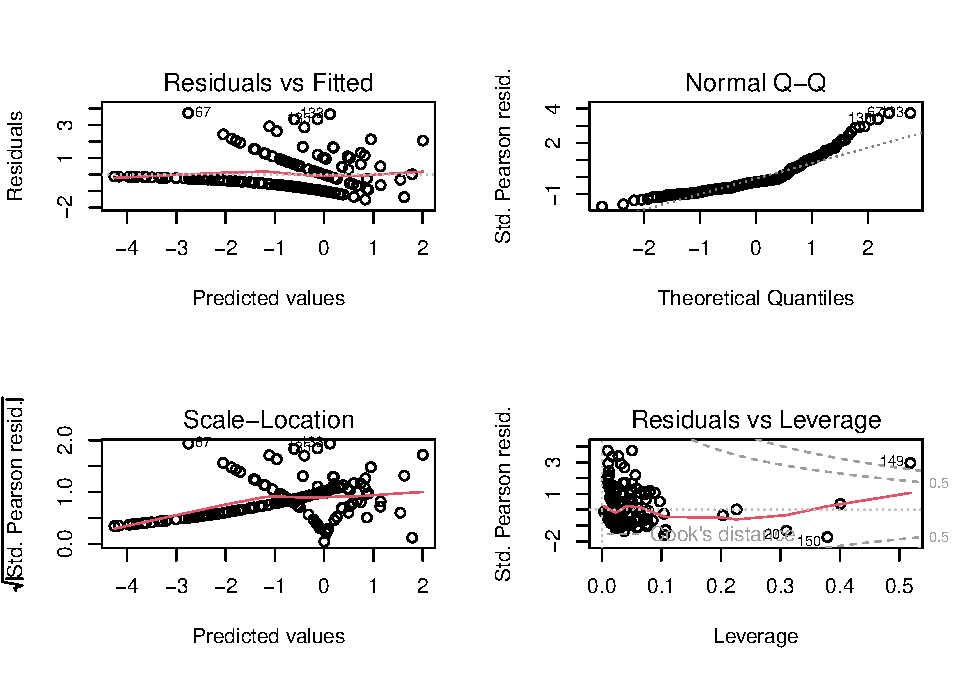
\includegraphics{Report_files/figure-latex/better model-1.pdf}

\emph{Poisson mixed model} To improve the model, we decide to fit a
mixed model. Indeed, by doing some variable selection with AIC or BIC,
one always obtain in the end Tunnel and Company due to their
heterogeneity. But, it isn't reasonable to consider that Fires depend
more on the company or the tunnel itself than paramters that define the
tunnel, that is to say the number of lanes, its length \ldots{}\\
The idea here is then to consider random and fixed effects on the
variables that were significant previously :\\
\emph{random : Tunnel, Company, }fixed : log(Traffic), HGV, Urban, Type,
log(Length), Limit, SlopeType, Width\\

\begin{verbatim}
## Warning: le package 'lme4' a été compilé avec la version R 4.2.2
\end{verbatim}

\begin{verbatim}
## Le chargement a nécessité le package : Matrix
\end{verbatim}

\begin{verbatim}
## Warning: le package 'Matrix' a été compilé avec la version R 4.2.2
\end{verbatim}

\begin{verbatim}
## 
## Attachement du package : 'Matrix'
\end{verbatim}

\begin{verbatim}
## Les objets suivants sont masqués depuis 'package:tidyr':
## 
##     expand, pack, unpack
\end{verbatim}

\begin{verbatim}
## Generalized linear mixed model fit by maximum likelihood (Laplace
##   Approximation) [glmerMod]
##  Family: poisson  ( log )
## Formula: Fires ~ log(Traffic) + HGV + log(Length) + (1 | Tunnel)
##    Data: Fires
## 
##      AIC      BIC   logLik deviance df.resid 
##    362.6    378.3   -176.3    352.6      165 
## 
## Scaled residuals: 
##     Min      1Q  Median      3Q     Max 
## -1.8249 -0.6091 -0.3277  0.3921  2.5358 
## 
## Random effects:
##  Groups Name        Variance Std.Dev.
##  Tunnel (Intercept) 0.322    0.5675  
## Number of obs: 170, groups:  Tunnel, 92
## 
## Fixed effects:
##              Estimate Std. Error z value Pr(>|z|)    
## (Intercept)  -21.6162     3.0211  -7.155 8.36e-13 ***
## log(Traffic)   0.8663     0.1304   6.641 3.11e-11 ***
## HGV            5.2058     1.4834   3.509 0.000449 ***
## log(Length)    0.6222     0.1603   3.882 0.000103 ***
## ---
## Signif. codes:  0 '***' 0.001 '**' 0.01 '*' 0.05 '.' 0.1 ' ' 1
## 
## Correlation of Fixed Effects:
##             (Intr) lg(Tr) HGV   
## log(Traffc) -0.941              
## HGV         -0.238  0.387       
## log(Length) -0.568  0.261 -0.352
\end{verbatim}

Then with company

\begin{verbatim}
## Generalized linear mixed model fit by maximum likelihood (Laplace
##   Approximation) [glmerMod]
##  Family: poisson  ( log )
## Formula: Fires ~ log(Traffic) + HGV + log(Length) + (1 | Company)
##    Data: Fires
## 
##      AIC      BIC   logLik deviance df.resid 
##    367.1    382.8   -178.6    357.1      165 
## 
## Scaled residuals: 
##     Min      1Q  Median      3Q     Max 
## -1.8326 -0.6663 -0.3322  0.3232  3.6168 
## 
## Random effects:
##  Groups  Name        Variance Std.Dev.
##  Company (Intercept) 0.09815  0.3133  
## Number of obs: 170, groups:  Company, 25
## 
## Fixed effects:
##              Estimate Std. Error z value Pr(>|z|)    
## (Intercept)  -21.9744     2.6301  -8.355  < 2e-16 ***
## log(Traffic)   0.8491     0.1116   7.610 2.75e-14 ***
## HGV            5.1012     1.2166   4.193 2.75e-05 ***
## log(Length)    0.7334     0.1485   4.940 7.80e-07 ***
## ---
## Signif. codes:  0 '***' 0.001 '**' 0.01 '*' 0.05 '.' 0.1 ' ' 1
## 
## Correlation of Fixed Effects:
##             (Intr) lg(Tr) HGV   
## log(Traffc) -0.926              
## HGV         -0.186  0.400       
## log(Length) -0.589  0.248 -0.463
\end{verbatim}

With both

\begin{verbatim}
## Generalized linear mixed model fit by maximum likelihood (Laplace
##   Approximation) [glmerMod]
##  Family: poisson  ( log )
## Formula: Fires ~ log(Traffic) + HGV + log(Length) + (1 | Company) + (1 |  
##     Tunnel)
##    Data: Fires
## 
##      AIC      BIC   logLik deviance df.resid 
##    364.2    383.0   -176.1    352.2      164 
## 
## Scaled residuals: 
##     Min      1Q  Median      3Q     Max 
## -1.8429 -0.6161 -0.3186  0.3640  2.6063 
## 
## Random effects:
##  Groups  Name        Variance Std.Dev.
##  Tunnel  (Intercept) 0.27296  0.5225  
##  Company (Intercept) 0.05001  0.2236  
## Number of obs: 170, groups:  Tunnel, 92; Company, 25
## 
## Fixed effects:
##              Estimate Std. Error z value Pr(>|z|)    
## (Intercept)  -22.0957     3.1826  -6.943 3.85e-12 ***
## log(Traffic)   0.8757     0.1353   6.471 9.74e-11 ***
## HGV            5.1493     1.5076   3.416 0.000636 ***
## log(Length)    0.6653     0.1757   3.786 0.000153 ***
## ---
## Signif. codes:  0 '***' 0.001 '**' 0.01 '*' 0.05 '.' 0.1 ' ' 1
## 
## Correlation of Fixed Effects:
##             (Intr) lg(Tr) HGV   
## log(Traffc) -0.934              
## HGV         -0.215  0.377       
## log(Length) -0.593  0.272 -0.358
\end{verbatim}

\hypertarget{accidents}{%
\subsection{Accidents}\label{accidents}}

We fit a Poisson model since we have count data.\\

\emph{Without random effects}\\

We first perform a forward and backward selection using the funtion
stepCriterion from the package glmtoolbox. The final model includes the
following variables : log(Traffic), SlopeType, log(Length), Limit, Type,
Width, Direction, Slope, HGV.

\begin{verbatim}
## Warning: le package 'glmtoolbox' a été compilé avec la version R 4.2.2
\end{verbatim}

\begin{verbatim}
## 
## Attachement du package : 'glmtoolbox'
\end{verbatim}

\begin{verbatim}
## L'objet suivant est masqué depuis 'package:boot':
## 
##     envelope
\end{verbatim}

\begin{verbatim}
## 
##        Family:  poisson 
## Link function:  log 
## 
## Initial model:
## ~ 1 
## 
## 
## Step 0 :
##                 df     AIC     BIC adj.R-squared P(Chisq>)(*)
## + log(Traffic)   1  8223.7  8233.8        0.4056    < 2.2e-16
## + SlopeType      4  8562.5  8587.8        0.3695    < 2.2e-16
## + Urban          1  8848.3  8858.4        0.3410    < 2.2e-16
## + Lanes          1 10517.3 10527.4        0.1684    < 2.2e-16
## + HGV            1 11085.3 11095.4        0.1096    < 2.2e-16
## + Limit          1 11143.8 11153.9        0.1035    < 2.2e-16
## + Type           1 11367.0 11377.1        0.0805    < 2.2e-16
## + Width          1 11702.0 11712.1        0.0458    < 2.2e-16
## + Direction      1 12125.5 12135.7        0.0020    1.565e-07
## + Slope          1 12132.7 12142.8        0.0013    5.805e-06
## <none>             12151.2 12156.3        0.0000             
## + log(Length)    1 12152.1 12162.2       -0.0007       0.2784
## 
## Step 1 : + log(Traffic) 
## 
##                 df    AIC    BIC adj.R-squared P(Chisq>)(*)
## + SlopeType      4 7104.6 7134.9        0.5205    < 2.2e-16
## + log(Length)    1 7713.2 7728.3        0.4581    < 2.2e-16
## + Limit          1 7803.6 7818.7        0.4488    < 2.2e-16
## + Urban          1 7916.9 7932.1        0.4371    < 2.2e-16
## + Width          1 8008.2 8023.3        0.4276    < 2.2e-16
## + HGV            1 8060.7 8075.9        0.4222    < 2.2e-16
## + Direction      1 8177.3 8192.5        0.4101    4.184e-12
## + Type           1 8186.6 8201.7        0.4091    1.880e-09
## + Slope          1 8211.2 8226.4        0.4066    0.0001392
## <none>             8223.7 8233.8        0.4056             
## + Lanes          1 8224.3 8239.4        0.4052    0.2264926
## 
## Step 2 : + SlopeType 
## 
##                 df    AIC    BIC adj.R-squared P(Chisq>)(*)
## + log(Length)    1 6764.5 6799.9        0.5556    < 2.2e-16
## + Limit          1 6861.7 6897.1        0.5456    < 2.2e-16
## + Urban          1 6931.4 6966.8        0.5383    < 2.2e-16
## + Width          1 6986.7 7022.1        0.5326    < 2.2e-16
## + HGV            1 6987.0 7022.4        0.5325    < 2.2e-16
## + Direction      1 7068.5 7103.9        0.5241    7.917e-10
## + Lanes          1 7075.2 7110.6        0.5234    2.678e-08
## + Slope          1 7094.3 7129.7        0.5214    0.0004544
## <none>             7104.6 7134.9        0.5205             
## + Type           1 7105.1 7140.5        0.5203    0.2249684
## - log(Traffic)   1 8562.5 8587.8        0.3695    < 2.2e-16
## 
## Step 3 : + log(Length) 
## 
##                 df    AIC    BIC adj.R-squared P(Chisq>)(*)
## + Limit          1 6360.0 6400.5        0.5975    < 2.2e-16
## + HGV            1 6569.7 6610.2        0.5757    < 2.2e-16
## + Urban          1 6577.7 6618.1        0.5749    < 2.2e-16
## + Width          1 6682.3 6722.8        0.5640    < 2.2e-16
## + Direction      1 6705.0 6745.5        0.5617    5.773e-15
## + Lanes          1 6744.2 6784.6        0.5576    2.616e-06
## + Type           1 6745.5 6786.0        0.5574    8.228e-06
## + Slope          1 6753.0 6793.4        0.5567     0.000234
## <none>             6764.5 6799.9        0.5556             
## - SlopeType      4 7713.2 7728.3        0.4581    < 2.2e-16
## - log(Traffic)   1 8423.6 8453.9        0.3836    < 2.2e-16
## 
## Step 4 : + Limit 
## 
##                 df    AIC    BIC adj.R-squared P(Chisq>)(*)
## + Type           1 6180.9 6226.4        0.6160    < 2.2e-16
## + HGV            1 6317.5 6363.0        0.6018    1.531e-10
## + Direction      1 6322.3 6367.8        0.6013    3.371e-10
## + Urban          1 6333.9 6379.4        0.6001    1.274e-07
## + Slope          1 6350.4 6395.9        0.5984    0.0006543
## + Lanes          1 6356.8 6402.3        0.5977    0.0218612
## + Width          1 6357.5 6403.0        0.5977    0.0324202
## <none>             6360.0 6400.5        0.5975             
## - log(Length)    1 6861.7 6897.1        0.5456    < 2.2e-16
## - SlopeType      4 7319.1 7339.3        0.4987    < 2.2e-16
## - log(Traffic)   1 8072.2 8107.6        0.4198    < 2.2e-16
## 
## Step 5 : + Type 
## 
##                 df    AIC    BIC adj.R-squared P(Chisq>)(*)
## + Width          1 6103.5 6154.1        0.6240    < 2.2e-16
## + Direction      1 6154.6 6205.2        0.6186    1.165e-07
## + HGV            1 6166.6 6217.2        0.6174    8.133e-05
## + Urban          1 6170.0 6220.5        0.6170    0.0003444
## + Slope          1 6170.6 6221.2        0.6170    0.0004675
## <none>             6180.9 6226.4        0.6160             
## + Lanes          1 6181.9 6232.4        0.6158    0.3223516
## - Limit          1 6745.5 6786.0        0.5574    < 2.2e-16
## - log(Length)    1 6821.3 6861.8        0.5496    < 2.2e-16
## - SlopeType      4 6939.6 6964.9        0.5378    < 2.2e-16
## - log(Traffic)   1 7514.0 7554.4        0.4775    < 2.2e-16
## 
## Step 6 : + Width 
## 
##                 df    AIC    BIC adj.R-squared P(Chisq>)(*)
## + Direction      1 6084.4 6140.0        0.6258    4.615e-06
## + Slope          1 6093.1 6148.7        0.6249    0.0004195
## + HGV            1 6095.5 6151.2        0.6247    0.0019430
## + Urban          1 6100.3 6155.9        0.6242    0.0231956
## + Lanes          1 6102.1 6157.7        0.6240    0.0650175
## <none>             6103.5 6154.1        0.6240             
## - Type           1 6357.5 6403.0        0.5977    < 2.2e-16
## - Limit          1 6577.4 6622.9        0.5748    < 2.2e-16
## - log(Length)    1 6704.4 6749.9        0.5615    < 2.2e-16
## - SlopeType      4 6753.2 6783.6        0.5570    < 2.2e-16
## - log(Traffic)   1 7257.5 7303.0        0.5040    < 2.2e-16
## 
## Step 7 : + Direction 
## 
##                 df    AIC    BIC adj.R-squared P(Chisq>)(*)
## + Slope          1 6073.4 6134.1        0.6269    0.0003061
## + HGV            1 6076.3 6136.9        0.6266    0.0017565
## + Urban          1 6080.7 6141.3        0.6261    0.0165833
## <none>             6084.4 6140.0        0.6258             
## + Lanes          1 6084.7 6145.4        0.6257    0.1923116
## - Width          1 6154.6 6205.2        0.6186    < 2.2e-16
## - Type           1 6320.3 6370.9        0.6014    < 2.2e-16
## - Limit          1 6531.0 6581.6        0.5794    < 2.2e-16
## - log(Length)    1 6696.0 6746.5        0.5623    < 2.2e-16
## - SlopeType      4 6741.6 6777.0        0.5580    < 2.2e-16
## - log(Traffic)   1 7258.6 7309.2        0.5036    < 2.2e-16
## 
## Step 8 : + Slope 
## 
##                 df    AIC    BIC adj.R-squared P(Chisq>)(*)
## + HGV            1 6065.3 6131.0        0.6276      0.00178
## + Urban          1 6069.8 6135.5        0.6271      0.01839
## <none>             6073.4 6134.1        0.6269             
## + Lanes          1 6074.8 6140.5        0.6266      0.43836
## - Direction      1 6093.1 6148.7        0.6249    3.412e-06
## - Width          1 6143.2 6198.8        0.6197    < 2.2e-16
## - Type           1 6309.0 6364.6        0.6024    < 2.2e-16
## - Limit          1 6520.0 6575.6        0.5804    < 2.2e-16
## - log(Length)    1 6689.5 6745.1        0.5628    < 2.2e-16
## - SlopeType      4 6726.4 6766.9        0.5594    < 2.2e-16
## - log(Traffic)   1 7253.1 7308.7        0.5040    < 2.2e-16
## 
## Step 9 : + HGV 
## 
##                 df    AIC    BIC adj.R-squared P(Chisq>)(*)
## <none>             6065.3 6131.0        0.6276             
## + Urban          1 6065.8 6136.5        0.6274    0.2209793
## + Lanes          1 6067.3 6138.0        0.6273    0.9555193
## - Slope          1 6076.3 6136.9        0.6266    0.0003102
## - Direction      1 6085.2 6145.9        0.6256    2.911e-06
## - Width          1 6129.1 6189.7        0.6211    4.441e-16
## - Type           1 6268.5 6329.1        0.6065    < 2.2e-16
## - Limit          1 6355.7 6416.4        0.5974    < 2.2e-16
## - log(Length)    1 6686.5 6747.1        0.5629    < 2.2e-16
## - SlopeType      4 6727.9 6773.4        0.5591    < 2.2e-16
## - log(Traffic)   1 7221.4 7282.1        0.5071    < 2.2e-16
## 
## Final model:
## ~ log(Traffic) + SlopeType + log(Length) + Limit + Type + Width + Direction + Slope + HGV 
## 
## ****************************************************************************
## (*) p-values of the Wald test
\end{verbatim}

Then, we build the model with those variables.\\

\begin{verbatim}
## 
## Call:
## glm(formula = Acc ~ log(Traffic) + SlopeType + log(Length) + 
##     Limit + Type + Width + Direction + Slope + HGV, family = poisson, 
##     data = Accidents)
## 
## Deviance Residuals: 
##     Min       1Q   Median       3Q      Max  
## -5.2931  -1.3919  -0.5937   0.7782   9.1138  
## 
## Coefficients:
##                            Estimate Std. Error z value Pr(>|z|)    
## (Intercept)               -9.953782   0.491001 -20.272  < 2e-16 ***
## log(Traffic)               0.636272   0.019181  33.172  < 2e-16 ***
## SlopeTypeBasin             0.893344   0.062644  14.261  < 2e-16 ***
## SlopeTypeUnknown           0.981202   0.073726  13.309  < 2e-16 ***
## SlopeTypeContinuous slope  0.128789   0.062946   2.046  0.04075 *  
## SlopeTypeRoof             -0.595817   0.110849  -5.375 7.66e-08 ***
## log(Length)                0.581543   0.023166  25.104  < 2e-16 ***
## Limit                     -0.018918   0.001069 -17.705  < 2e-16 ***
## TypeUnidirectional         0.961621   0.070419  13.656  < 2e-16 ***
## Width                     -0.635981   0.078212  -8.132 4.24e-16 ***
## DirectionDirection 2      -0.139262   0.029776  -4.677 2.91e-06 ***
## Slope                     -2.467565   0.684174  -3.607  0.00031 ***
## HGV                       -0.825490   0.264178  -3.125  0.00178 ** 
## ---
## Signif. codes:  0 '***' 0.001 '**' 0.01 '*' 0.05 '.' 0.1 ' ' 1
## 
## (Dispersion parameter for poisson family taken to be 1)
## 
##     Null deviance: 9676  on 1159  degrees of freedom
## Residual deviance: 3566  on 1147  degrees of freedom
## AIC: 6065.3
## 
## Number of Fisher Scoring iterations: 5
\end{verbatim}

Both AIC and deviance 3566.0272322 are quite big. Our variables are
significant at the usual 5\%.\\

\emph{With random effects}\\
We now want to adjust our Poisson model with random effects. As for the
dataset Fires, we consider :\\
\emph{random : Tunnel, Company,\\
}fixed : log(Traffic), SlopeType, log(Length), Limit, Type, Width,
Direction, Slope, HGV\\

The model doesn't converge if we use the same variables as for the model
without random effects. Indeed, by fitting the model with the exact same
setup, we obtain with a mixed model that SlopeType isn't significant,
nor HGV. We fit the model without those variables.\\

\begin{verbatim}
## Warning in log(Traffic): Production de NaN
\end{verbatim}

\begin{verbatim}
## Warning in log(Length): Production de NaN
\end{verbatim}

\begin{verbatim}
## Warning in log(Traffic): Production de NaN
\end{verbatim}

\begin{verbatim}
## Warning in log(Length): Production de NaN
\end{verbatim}

\begin{verbatim}
## boundary (singular) fit: see help('isSingular')
\end{verbatim}

\begin{verbatim}
## Generalized linear mixed model fit by maximum likelihood (Laplace
##   Approximation) [glmerMod]
##  Family: poisson  ( log )
## Formula: Acc ~ log(Traffic) + Slope + HGV + log(Length) + Limit + Type +  
##     (1 | Tunnel) + (1 | Company)
##    Data: Accidents_new
## 
##      AIC      BIC   logLik deviance df.resid 
##    433.0    449.4   -207.5    415.0       37 
## 
## Scaled residuals: 
##     Min      1Q  Median      3Q     Max 
## -3.5255 -1.4892 -0.2783  1.1671  5.6802 
## 
## Random effects:
##  Groups  Name        Variance Std.Dev.
##  Tunnel  (Intercept) 0        0       
##  Company (Intercept) 0        0       
## Number of obs: 46, groups:  Tunnel, 5; Company, 3
## 
## Fixed effects:
##                    Estimate Std. Error z value Pr(>|z|)    
## (Intercept)         2.93005    0.77297   3.791  0.00015 ***
## log(Traffic)        0.14460    0.15638   0.925  0.35514    
## Slope               0.35116    0.07191   4.883 1.04e-06 ***
## HGV                 1.39433    0.12498  11.157  < 2e-16 ***
## log(Length)         0.42990    0.16664   2.580  0.00989 ** 
## Limit              -1.33698    0.27916  -4.789 1.67e-06 ***
## TypeUnidirectional  0.99629    0.59720   1.668  0.09526 .  
## ---
## Signif. codes:  0 '***' 0.001 '**' 0.01 '*' 0.05 '.' 0.1 ' ' 1
## 
## Correlation of Fixed Effects:
##             (Intr) lg(Tr) Slope  HGV    lg(Ln) Limit 
## log(Traffc)  0.884                                   
## Slope        0.179  0.105                            
## HGV         -0.412 -0.413 -0.009                     
## log(Length)  0.760  0.610  0.171 -0.056              
## Limit       -0.567 -0.539 -0.088 -0.306 -0.876       
## TypUndrctnl -0.947 -0.883 -0.150  0.497 -0.515  0.340
## optimizer (Nelder_Mead) convergence code: 0 (OK)
## boundary (singular) fit: see help('isSingular')
\end{verbatim}

\emph{Negative binomial}\\
With random effects\\
Still a problem with convergence\ldots{} so\ldots{}\\

\begin{verbatim}
## Warning in checkConv(attr(opt, "derivs"), opt$par, ctrl = control$checkConv, :
## Model failed to converge with max|grad| = 0.0536059 (tol = 0.002, component 1)
\end{verbatim}

\begin{verbatim}
## Warning in checkConv(attr(opt, "derivs"), opt$par, ctrl = control$checkConv, : Model is nearly unidentifiable: very large eigenvalue
##  - Rescale variables?;Model is nearly unidentifiable: large eigenvalue ratio
##  - Rescale variables?
\end{verbatim}

\begin{verbatim}
## Warning in checkConv(attr(opt, "derivs"), opt$par, ctrl = control$checkConv, :
## Model failed to converge with max|grad| = 0.227163 (tol = 0.002, component 1)
\end{verbatim}

\begin{verbatim}
## Warning in checkConv(attr(opt, "derivs"), opt$par, ctrl = control$checkConv, : Model is nearly unidentifiable: very large eigenvalue
##  - Rescale variables?;Model is nearly unidentifiable: large eigenvalue ratio
##  - Rescale variables?
\end{verbatim}

\begin{verbatim}
## Warning in optTheta(g1, interval = interval, tol = tol, verbose = verbose, : Model is nearly unidentifiable: very large eigenvalue
##  - Rescale variables?;Model is nearly unidentifiable: large eigenvalue ratio
##  - Rescale variables?
\end{verbatim}

\begin{verbatim}
## Generalized linear mixed model fit by maximum likelihood (Laplace
##   Approximation) [glmerMod]
##  Family: Negative Binomial(2.6335)  ( log )
## Formula: Acc ~ log(Traffic) + log(Length) + Limit + Type + Width + Direction +  
##     Slope + (1 | Tunnel) + (1 | Company)
##    Data: Accidents
## 
##      AIC      BIC   logLik deviance df.resid 
##   4667.5   4723.1  -2322.8   4645.5     1149 
## 
## Scaled residuals: 
##     Min      1Q  Median      3Q     Max 
## -1.4952 -0.7333 -0.2245  0.4812  6.4009 
## 
## Random effects:
##  Groups  Name        Variance Std.Dev.
##  Tunnel  (Intercept) 0.2702   0.5198  
##  Company (Intercept) 0.1042   0.3229  
## Number of obs: 1160, groups:  Tunnel, 92; Company, 25
## 
## Fixed effects:
##                       Estimate Std. Error z value Pr(>|z|)    
## (Intercept)          -9.687313   2.146351  -4.513 6.38e-06 ***
## log(Traffic)          0.699202   0.079996   8.741  < 2e-16 ***
## log(Length)           0.526491   0.092307   5.704 1.17e-08 ***
## Limit                -0.016321   0.004772  -3.420 0.000625 ***
## TypeUnidirectional    0.992527   0.245167   4.048 5.16e-05 ***
## Width                -1.001488   0.415964  -2.408 0.016056 *  
## DirectionDirection 2 -0.010868   0.057745  -0.188 0.850716    
## Slope                -2.667046   1.105406  -2.413 0.015834 *  
## ---
## Signif. codes:  0 '***' 0.001 '**' 0.01 '*' 0.05 '.' 0.1 ' ' 1
## 
## Correlation of Fixed Effects:
##             (Intr) lg(Tr) lg(Ln) Limit  TypUnd Width  DrctD2
## log(Traffc) -0.747                                          
## log(Length) -0.320  0.100                                   
## Limit       -0.129  0.063 -0.024                            
## TypUndrctnl  0.340 -0.420  0.342 -0.225                     
## Width       -0.721  0.246 -0.099 -0.096 -0.373              
## DrctnDrctn2  0.048 -0.052 -0.045 -0.060  0.048 -0.014       
## Slope        0.021 -0.005 -0.015 -0.015  0.002 -0.015 -0.066
## optimizer (Nelder_Mead) convergence code: 0 (OK)
## Model is nearly unidentifiable: very large eigenvalue
##  - Rescale variables?
## Model is nearly unidentifiable: large eigenvalue ratio
##  - Rescale variables?
\end{verbatim}

\hypertarget{discussion}{%
\section{Discussion}\label{discussion}}

QQplots, analyse modèles, ce qu'on aurait pu améliorer

\hypertarget{references}{%
\section{References}\label{references}}

\end{document}
